\chapter{Background}

\section{Definition of terms}

To prevent missunderstandings and confusion, the following subsections 2.1.1 - 2.1.x will define some terminoligy which will be mandatory for the understanding of certain areas of this thesis.


\subsection{Deep Zoom Image Format}

The Deep Zoom Image Format (.dzi)\nomenclature{.dzi}{Deep Zoom Image Format} is an xml-based file format maintained by Microsoft to improve performance and quality in the handling of large image files. For this purpose an image is represented in a tiled pyramid (see fig. 2.1).
			
\begin{figure}[!htbp]
	\begin{center}
		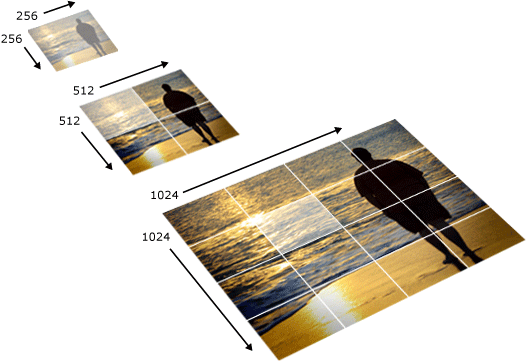
\includegraphics[scale=0.5]{img/dzi_pyramid.png}
		\caption{3 consecutive levels of a .dzi image (source: https://i-msdn.sec.s-msft.com/dynimg/IC141135.png)}
		\label{fig:fig2.1}
	\end{center}
\end{figure}

As seen in fig. 2.1 there are multiple versions of a single image in different resolutions. Each resolution in the pyramid is called a \emph{level}. At each level the image is scaled down by the factor 4 (2 in each dimension). Furthermore, the image gets tiled up into $256^2$ tiles (256 in each dimension)\cite{web:dzi}.

If a viewer wants to view a certain area of the image (e.g. the highlighted tile in the last image in fig. 2.1), only the corresponding tiles need to be loaded. This saves large amounts of bandwidth and memory. The same goes for a viewer, who is zoomed out very far. In such a view the full level of detail isn't needed, so that a version from a lower level can be loaded.

A .dzi file consists of two parts: a describing .xml file\footnote{Frameworks like \emph{OpenSeaDragon} also support further formats, such as .json.} and a folder with more subfolder. Each subfolder describes a level and as such contains all the tiles for that particular level.
\newpage

\subsection{Microservice}

The concept of microservices is to seperate one monolithic software construct into several smaller, modular pieces of software. According to \cite{Wolff16}, the idea of microservices is not new, but can be found in the UNIX philosophy. Three basic ideas are stated in \cite{Wolff16}:

\begin{itemize}
	\item A program should fulfill only one task, and it should do it well.
	\item Programs should be able to work together.
	\item Besides, the programs should use a universal interface.
\end{itemize}

As such, microservices are a modularization concept. However, they differ from other concepts, since they are independet from each other. This is a trait, other modularization concepts usually lack. As a result, changes in one microservice don't bring up the necessity of deploying the whole product again but just the one service.

Because of their inherent traits, microservices need to be their own processes in one way or another, may it be as an actual operating system process or as e.g. a docker container\footnote{Docker is a tool, which enables software to be wrapped up in so called "'containers"'. Those containers are a complete, but stripped down, filesystem containing everything the software needs to run (e.g. source code, runtime environment, system tools and libraries, ...). See \url{https://www.docker.com/what-docker}}.

One big advantage of this modularization is that each service can be written in a different programming language, using different frameworks and tools. Furthermore, each microservice can bring along its own support services and data storages, like data bases. It is imperative for the concept of modularization, however, that each microservice has its own storage of which it is in charge of.

A disadvantage of this modularization is, that inter process communication becomes a necessity. However, there are different approaches with which microservices can communicate. \cite{Wolff16} suggests the following:

\begin{itemize}
	\item communication via protocols like REST
	\item an HTML user interfaces with links to other microservices
	\item data replication
\end{itemize}

It is important to define how and with which technology to communicate with, when adressing each microservices to ensure that this particular one can actually be reached with the defined method.


\subsection{Machine Learning}
\subsection{Neural Networks}
\section{Process chain}
\subsection{Description}
\subsection{Definition of Conversion Service}
\subsection{Definition of Annotation Service}
\subsection{Definition of Tesselation Service}